\paragraph{Setup: turning math objects into \code{deal.II} objects}

The setup process has four parts:
\begin{enumerate}
    \item \important{Mesh $+$ boundary IDs}
    \begin{lstlisting}[language=C++]
// Create the mesh.
{
    printf("Initializing the mesh\n");
    GridGenerator::subdivided_hyper_cube(
        mesh, N + 1, 0.0, 1.0, true
    );
    printf(
        "  Number of elements = %d\n",
        mesh.n_active_cells()
    );

    // Write the mesh to file.
    const std::string mesh_file_name = "mesh-" +
        std::to_string(N + 1) + ".vtk";
    const GridOut grid_out;
    std::ofstream grid_out_file(mesh_file_name);
    grid_out.write_vtk(mesh, grid_out_file);
    printf("  Mesh saved to %s\n", mesh_file_name.c_str());
}\end{lstlisting}
    The mesh is the scaffold that turns the continuous PDE on $\Omega$ into a finite-dimensional problem we can actually compute.
    \begin{itemize}
        \item \textbf{\emph{Math picture (what we want)}}
        \begin{itemize}
            \item Domain: the closed interval $\left[0,1\right]$.
            \item Partition (mesh): split $\left[0,1\right]$ into small sub-intervals (cells/elements). If we have $N$ cells, the vertices are $N+1$ points: $x_0=0 < x_1 < \dots < x_M=1$.
            \item Boundary: the two endpoint $x=0$ (left) and $x=1$ (right).
        \end{itemize}

        \item \textbf{\emph{\code{deal.II} objects (how it represents that picture)}}. \code{Triangulation<dim>} \textbf{is the mesh container} (cells $+$ faces $+$ links). The name ``triangulation'' comes from numerical PDE jargon: \emph{any} partition of a domain into simple elements (segments in 1D, triangles/quads in 2D, tets/hexes in 3D) is often called a ``triangulation'', even when the cells aren't literal triangles.
        
        \textcolor{Green3}{\faIcon{question-circle} \textbf{What does a Triangulation store?}} Geometry and topology of the mesh. It stores \textbf{vertices} (coordinates) and \textbf{cells} (their vertex indices), plus who's adjacent to whom (\textbf{links}). This is the scaffold on which we place basis functions and do integrals cell-by-cell.

        In 1D:
        \begin{itemize}
            \item A \textbf{cell} is an interval $\left[x_{i}, x_{i+1}\right]$;
            \item A \textbf{face} is a 0-D endpoint (vertex).
            \item \textbf{Boundary faces} are endpoints located on the boundary of the domain (here, just $x=0$ and $x=1$).
        \end{itemize}
    \end{itemize}
    In summary, it creates a 1D mesh on $\left[0,1\right]$ with $N + 1$ \textbf{elements} (so $N+2$ \textbf{nodes} for $r=1$). The last boolean parameter in the \code{subdivided\_hyper\_cube} invocation means that the colorize parameter is set to true (\code{colorize=true}), and assigns \textbf{boundary id 0} to $x=0$ and \textbf{id 1} to $x=1$. We'll use these IDs to impose Dirichlet in \code{assemble()}.

    \textcolor{Green3}{\faIcon{question-circle} \textbf{Why VTK export now (\code{write\_vtk})?}} So we can see the mesh and quickly catch wrong counts/IDs.

    \textcolor{Green3}{\faIcon{tools} \textbf{API Meaning}}
    \begin{enumerate}
        \item \code{subdivided\_hyper\_cube(mesh, M, a, b, colorize)}. In 1D, this creates a line segment $\left[a,b\right]$ split into $M$ equal cells. Here, $M = N + 1$, $a = 0.0$ and $b=1.0$. So we get $N+1$ intervals.
        
        \item \textbf{What does ``active'' mean?} Triangulations can be adaptively refined, creating a tree of parent/child cells. ``\textbf{Active cells}'' are the \emph{leaves} (the current mesh we compute on). Immediately after creation, every cell is active.
        
        \item \code{colorize = true} (crucial for boundary IDs)
        \begin{itemize}
            \item If \code{false}, \emph{all} boundary faces get the \textbf{same} \code{boundary\_id} (typically 0). That's OK for ``Dirichlet everywhere $= 0$'', but useless for different BCs on different sides.
            \item If \code{true}, \code{deal.II} assigns \textbf{distinct IDs} per ``side'' of the hypercube:
            \begin{itemize}
                \item In 1D:
                \begin{itemize}
                    \item \textbf{ID 0}: left endpoint $x=a$ (the ``minus'' face along $x$).
                    \item \textbf{ID 1}: right endpoint $x=b$ (the ``plus'' face along $x$).
                \end{itemize}
                \item In 2D:
                \begin{itemize}
                    \item ID 0: $-x$ (left)
                    \item ID 1: $+x$ (right)
                    \item ID 2: $-y$ (bottom)
                    \item ID 3: $+y$ (top)
                \end{itemize}
                \item In 3D:
                \begin{itemize}
                    \item ID 0: $-x$
                    \item ID 1: $+x$
                    \item ID 2: $-y$
                    \item ID 3: $+y$
                    \item ID 4: $-z$
                    \item ID 5: $+z$
                \end{itemize}
            \end{itemize}
        \end{itemize}
        Because the IDs are distinct, we \emph{could} assign different functions to 0 and 1 if we wanted mixed boundary conditions.

        \textcolor{Green3}{\faIcon{question-circle} \textbf{Why is it called \code{colorize}?}} In the context of meshing, ``\code{colorize}'' refers to labeling parts with distinct tags. \code{deal.II} uses integer tags called \code{boundary\_id}. Setting \code{colorize=true} tells the generator to \textbf{color} each side with a different \code{boundary\_id} so we can target them individually for boundary conditions.
    \end{enumerate}


%%%%%%%%%%%%%%%%%%%%%%%%%%%%%%%%%%%%%%%%%%%%%%%%%%%%%%%%%%%
    

    \newpage
    \item \important{Finite element $+$ quadrature}
    \begin{lstlisting}[language=C++]
// Initialize the finite element space.
{
    printf("Initializing the finite element space\n");

    // Finite elements in one dimension are obtained with
    // the FE_Q class (which for higher dimensions represents
    // hexahedral finite elements).
    // In higher dimensions, we must use FE_Q for
    // hexahedral elements or FE_SimplexP for tetrahedral
    // elements. They are both derived from
    // FiniteElement, so that the code is generic.
    fe = std::make_unique<FE_Q<dim>>(r);

    printf(
        "  Degree                     = %d\n",
        fe->degree
    );
    printf(
        "  DoFs per cell              = %d\n",
        fe->dofs_per_cell
    );

    // Construct the quadrature formula of the
    // appropriate degree of exactness.
    // This formula integrates exactly the mass
    // matrix terms (i.e. products of basis functions).
    quadrature = std::make_unique<QGauss<dim>>(r + 1);

    printf(
        "  Quadrature points per cell = %d\n",
        quadrature->size()
    );
}\end{lstlisting}
    \textcolor{Green3}{\faIcon{question-circle} \textbf{Finite element (\code{FE\_Q}): What does the math need?}} We decide to approximate the solution in a space:
    \begin{equation*}
        V_{h} = \left\{v\in C^0([0,1]) \;|\; v|_K \in \mathbb P_r \ \text{for every cell }K\in\mathcal T_h\right\}
    \end{equation*}
    So on \textbf{each cell} $K$ we use polynomials of degree $r$, and we glue cells together with continuity at the nodes.

    \textcolor{Green3}{\faIcon{question-circle} \textbf{Finite element (\code{FE\_Q}): How \code{deal.II represents that}}}
    \begin{itemize}
        \item \code{FE\_Q<dim>(r)}: \textbf{Lagrange $\mathbb{P}_{r}$ elements} on a (hyper)cube cell (Q $=$ hypercube elements, segments in 1D, quads in 2D, hexes in 3D). In 1D, the reference cell is $\left[0,1\right]$. The \textbf{local basis} are the Lagrange shape functions $\left\{\phi_{i}\right\}_{i=0}^{r}$ that are 1 at the one node and 0 at the others (nodal basis).
        
        In other words, \code{FE\_Q(r)} says ``on each cell, use $r+1$ nodal polynomials and glue cells continuously''.
        \item \textbf{DoFs per cell} in 1D: \code{fe -> dofs\_per\_cell = r + 1}. For example, with $r=1$, 2 DoFs per cell (endpoints); $r=2$ 3 DoFs per cell (endpoints $+$ midpoint).
        \item \textbf{Global DoFs} with $M$ cells and degree $r$ in 1D:
        \begin{equation*}
            N_{\text{dofs}} = M \cdot r + 1
        \end{equation*}
        Because adjacent cells share nodes. In our code, $M = N+1$, so for $r=1$: $N_{\text{dofs}} = \left(N+1\right) \cdot 1 + 1 = N + 2$.
    \end{itemize}

    \textcolor{Green3}{\faIcon{question-circle} \textbf{Quadrature (\code{QGauss}): What does the math need?}} For Poisson, on each cell $K$ we must compute:
    \begin{itemize}
        \item \textbf{Stiffness}: $A_{ij}^K = \displaystyle\int_K \mu \cdot \phi_{j}' \cdot \phi_{i}' \,\mathrm{d}x$
        \item \textbf{Load}: $f_{i}^{K} = \displaystyle\int_{K} f \, \phi_{i} \, \mathrm{d}x$
    \end{itemize}
    These are \textbf{integrals of polynomials (or polynomials $\times$ coefficient)} over $K$. We approximate them with Gauss-Legendre quadrature.

    \textcolor{Green3}{\faIcon{question-circle} \textbf{Quadrature (\code{QGauss}): How \code{deal.II represents that.}}}
    
    In \code{deal.II}, \code{QGauss} is a \textbf{numerical integration rule}: it tells \code{deal.II} which points $x_{q}$ to sample on a cell and \emph{which weights} $w_{q}$ to multiply by, so that an integral is approximated by a weighted sum
    \begin{equation*}
        \displaystyle\int_{K} g(x)\,\mathrm{d}x \;\approx\; \displaystyle\sum_{q=1}^{n_q} g(x_q)\cdot w_q \;\;\;(\text{on cell }K)
    \end{equation*}
    Specifically, \textbf{Gauss-Legendre} with $n_{q}$ points is \textbf{exact} for all \textbf{polynomials up to degree $2n_{q}-1$} on an \textbf{interval}. That's why we like it for FEM on (hyper)cube cells.
    
    \code{QGauss} controls \textbf{how we integrate} on each cell during assembly (and post-processing): i.e., \textbf{how many sample points} inside the cell we use, and with which \textbf{weights}, to approximate integrals.
    \begin{itemize}
        \item \textbf{Triangulation / mesh}: how many cells, their size/shape, boundary tags. This \hl{sets where the domain is cut and how fine the grid is}.
        \item \textbf{Finite element \code{FE\_Q(r)}}: which basis we use on each cell (degree $r$, continuity). This \hl{sets how ``complex'' the polynomial we can represent per cell is}.
        \item \textbf{Quadrature \code{QGauss(n\_q)}}: how many \textbf{sample points} per cell we use to compute the integrals that build $A$ and $f$. This \hl{sets how accurately we evaluate those integrals, not the mesh, not the basis}.
    \end{itemize}
    \textcolor{Green3}{\faIcon{question-circle} \textbf{What does \code{QGauss} actually give us?}} For an interval (our 1D cell), \code{QGauss<1>(n\_q)} returns $n_{q}$ reference points and weights that are \textbf{exact for all polynomials up to degree} $2n_{q}-1$. 

    \textcolor{Red2}{\faIcon{exclamation-triangle} \textbf{Undershooting $n_{q}$.}} If we pick too few points, we'll get consistency/accuracy issues (quietly!). The standard rule is generally to use $r+1$.
    

%%%%%%%%%%%%%%%%%%%%%%%%%%%%%%%%%%%%%%%%%%%%%%%%%%%%%%%%%%%
    

    \newpage
    \item \important{DoFHandler: global numbering of unknowns}
    \begin{lstlisting}[language=C++]
// Initialize the DoF handler.
{
    printf("Initializing the DoF handler\n");

    // Initialize the DoF handler with the mesh
    // we constructed.
    dof_handler.reinit(mesh);

    // "Distribute" the degrees of freedom.
    // For a given finite element space,
    // initializes info on the control variables
    // (how many they are, where
    // they are collocated, their "global indices", ...).
    dof_handler.distribute_dofs(*fe);

    printf("  Number of DoFs = %d\n", dof_handler.n_dofs());
}\end{lstlisting}
    \textcolor{Green3}{\faIcon{question-circle} \textbf{What problem it solves (conceptually).}} After we pick the FE space $V_{h}$ with \code{FE\_Q<1>(r)} and we have a mesh $\mathcal{T}_{h}$, we need a \textbf{single global index} for every unknown (degree of freedom, DoF) in the problem. That global numbering is what lets us build the global vector $u, f$ and the sparse matrix $A$.
    \begin{itemize}
        \item \textbf{Locally (per cell)} we have $r+1$ shape functions $\left\{\phi_{i}\right\}_{i=0}^{r}$.
        \item \textbf{Globally} many of those DoFs are \textbf{shared} at interfaces (e.g., the right vertex of one cell is the left vertex of the next).
        \item The \textbf{DoFHandler} walks the mesh and \textbf{assign unique global indices} to those shared DoFs exactly once, so the global system reflects continuity correctly.
    \end{itemize}

    \textcolor{Green3}{\faIcon{question-circle} \textbf{What the two calls do}}
    \begin{lstlisting}[language=C++]
// attach to triangulation
dof_handler.reinit(mesh);
// assign global DoF indices using 'fe'
dof_handler.distribute_dofs(*fe);\end{lstlisting}
    \begin{itemize}
        \item \code{reinit(mesh)}: tells the handler which mesh to use.
        \item \code{distribute\_dofs(*fe)}: asks \code{fe} where DoFs live on each cell and then produces a global numbering that respects sharing across cell interfaces.
    \end{itemize}
    In general, \textbf{triangulation first}, \textbf{then DoFHandler}, \textbf{then distribute DoFs}, and only \emph{after that} we can build the sparsity pattern and allocate matrices/vectors.

    \textcolor{Green3}{\faIcon{question-circle} \textbf{How many DoFs do we get in 1D?}} Let $M$ be the number of cells (in our code $M = N + 1$). For \code{FE\_Q(r)} in 1D:
    \begin{equation*}
        \#\text{DoFs} \;=\; M \cdot r + 1 
    \end{equation*}
    The first cell contributes $r+1$ DoFs, and each subsequent cell contributes $r$ new ones (the interface node is shared), so:
    \begin{equation*}
        \left(r+1\right) + \left(M-1\right) \cdot r = Mr + 1
    \end{equation*}
    \begin{examplebox}[: A tiny concrete picture]
        If $r=1$ and $N=3$:
        \begin{itemize}
            \item Mesh: $M = N+1 = 4$ cells, nodes at $x_0=0, x_1, x_2, x_3, x_4=1$.
            \item Global DoFs (before BCs): indices $0,1,2,3,4$ (so \code{n\_dofs = 5 = N+2}).
            \item Cells and their local to global maps:
            \begin{itemize}
                \item Cell 0 $\left[x_{0}, x_{1}\right]$: local \code{(0, 1)} $\rightarrow$ global \code{(0, 1)}
                \item Cell 1 $\left[x_{1}, x_{2}\right]$: local \code{(0, 1)} $\rightarrow$ global \code{(1, 2)}
                \item Cell 2 $\left[x_{2}, x_{3}\right]$: local \code{(0, 1)} $\rightarrow$ global \code{(2, 3)}
                \item Cell 3 $\left[x_{3}, x_{4}\right]$: local \code{(0, 1)} $\rightarrow$ global \code{(3, 4)}
            \end{itemize}
            \item During assembly on Cell 1, for example, when we add \code{cell\_matrix(0, 1)} we write into global \code{A(1, 2)}; on Cell 2 the same local entry writes into \code{A(2, 3)}, etc. Shared nodes cause \textbf{sums} into the same rows/cols (that's how continuity/gluing shows up algebraically).
        \end{itemize}
    \end{examplebox}
    

%%%%%%%%%%%%%%%%%%%%%%%%%%%%%%%%%%%%%%%%%%%%%%%%%%%%%%%%%%%
    

    \item \important{Sparse structure $+$ algebra shells}
    \begin{lstlisting}[language=C++]
// Initialize the linear system.
{
    printf("Initializing the linear system\n");

    // First, we need to initialize the sparsity pattern.
    // This object describes the structure of the system
    // matrix (i.e. which entries are nonzero).
    // We use a DynamicSparsityPattern object to generate
    // the sparsity pattern, and then copy it into a
    // SparsityPattern object,
    // which is more efficient for computations.
    printf("  Initializing the sparsity pattern\n");
    DynamicSparsityPattern dsp(dof_handler.n_dofs());
    DoFTools::make_sparsity_pattern(dof_handler, dsp);
    sparsity_pattern.copy_from(dsp);

    // Then, we use the sparsity pattern to initialize
    // the system matrix
    printf("  Initializing the system matrix\n");
    system_matrix.reinit(sparsity_pattern);

    // Finally, we initialize the right-hand side and
    // solution vectors.
    printf("  Initializing the system right-hand side\n");
    system_rhs.reinit(dof_handler.n_dofs());
    printf("  Initializing the solution vector\n");
    solution.reinit(dof_handler.n_dofs());
}\end{lstlisting}
    The goal of this step is to encode \textbf{which pairs of DoFs can couple} (i.e., where $A_{ij}$ might be nonzero), and allocate the sparse matrix $A$ and vectors $f, u$ with the \textbf{right sizes and layout}.

    \textcolor{Green3}{\faIcon{book} \textbf{From FE connectivity $\rightarrow$ nonzero pattern.}} In FEM, DoFs are the unknowns (one per basis function). Two DoFs \textbf{couple} if their basis functions \textbf{overlap on at least one cell}. In the matrix $A$, this means the entry $A_{ij}$ \textbf{can be nonzero}. So the \textbf{sparsity pattern} is just the list of all index pairs $\left(i,j\right)$ where $A_{ij}$ might be nonzero. We \textbf{precompute} this once (fast) before assembly so the sparse matrix knows exactly which slots to allocate.

    \begin{examplebox}[: 1D]
        Let $r=1$, 4 cells and then $5$ DoFs. Cells (with their \textbf{global} DoFs):
        \begin{itemize}
            \item Cell 0: $[x_0,x_1]$ $\rightarrow$ DoFs (0,1)
            \item Cell 1: $[x_1,x_2]$ $\rightarrow$ DoFs (1,2)
            \item Cell 2: $[x_2,x_3]$ $\rightarrow$ DoFs (2,3)
            \item Cell 3: $[x_3,x_4]$ $\rightarrow$ DoFs (3,4)
        \end{itemize}
        Each cell has \textbf{2 local DoFs}: its left and right vertices. With 4 cells, we might have global DoFs $0,1,2,3,4$. The sparsity pattern it built by inserting \textbf{all pairs} from each cell's set $I \times I$:
        \begin{itemize}
            \item From cell 0: $(0,0)$, $(0,1)$, $(1,0)$, $(1,1)$
            \item From cell 1: $(1,1)$, $(1,2)$, $(2,1)$, $(2,2)$
            \item Etc.
        \end{itemize}
        Collecting unique pairs gives this \textbf{tridiagonal} pattern:
        \begin{equation*}
            \begin{bmatrix}
                \mathrm{x}  & \mathrm{x}    &               &               & \\
                \mathrm{x}  & \mathrm{x}    & \mathrm{x}    &               & \\
                            & \mathrm{x}    & \mathrm{x}    & \mathrm{x}    & \\
                            &               & \mathrm{x}    & \mathrm{x}    & \mathrm{x} \\
                            &               &               & \mathrm{x}    & \mathrm{x} \\
            \end{bmatrix}
        \end{equation*}
        Those x are the positions we \textbf{pre-allocate}. Later, assembly just \textbf{adds numbers} into these slots.
    \end{examplebox}

    \textcolor{Green3}{\faIcon{question-circle} \textbf{Why ``precompute'' the pattern?}} Making the sparse matrix grow on-the-fly is expensive and unsafe. Instead, we do:
    \begin{lstlisting}[language=C++]
DynamicSparsityPattern dsp(n_dofs);
for (each cell K) {
  I = global dof indices on K;
  for (i in I) for (j in I) dsp.add(i,j);  // mark possible nonzeros
}
sparsity_pattern.copy_from(dsp);
system_matrix.reinit(sparsity_pattern);    // allocate exact slots
    \end{lstlisting}
    Now assembly can do constant-time adds into known positions.

    \textcolor{Green3}{\faIcon{question-circle} \textbf{Why this structure?}}
    \begin{itemize}
        \item \textbf{Build the graph dynamically (cheap inserts)}: \code{DynamicSparsityPattern dsp(dof\_handler.n\_dofs());} The \textbf{sparsity pattern} tells us which entries of the global matrix may be non zero. This data structure is an insertion-friendly container. While we scan each cell and its local DoFs, we ``declare'' couplings $(i,j)$ by inserting them into \code{dsp}. Inserts are frequenti and irregular, so we need a structure that doesn't reallocate like crazy.
        
        \textcolor{Green3}{\faIcon{question-circle} \textbf{Why are we talking about graphs?}} \code{deal.II} never draws a graph, but under the hood uses an abstract adjacency graph of the sparse matrix:
        \begin{itemize}
            \item Vertices are DoFs (global unknown indices $0 \dots N-1$).
            \item Edges $(i,j)$ are potential nonzero $A_{ij}$ (i.e., DoF $i$ couples with DoF $j$ on at least one cell).
        \end{itemize}
        \code{DoFTools::make\_sparsity\_pattern(dof\_handler,dsp)} walks the mesh cell by cell, looks at the \textbf{local} DoFs on that cell, and for every pair $(i,j)$ in that local set, it marks an entry in \code{dsp}. That is literally building the \textbf{adjacency} of the global matrix, just not visually.

        \begin{examplebox}[: Graph 1D]
            For example, with $r = 1$ and a uniform mesh, the degrees of freedom (DoFs) are $0, 1, 2, 3$ and $4$ along the line. Cells: \code{[0, 1]}, \code{[1, 2]}, \code{[2, 3]}, \code{[3, 4]}. Each cell contributes couplings among its two DoFs:
            \begin{itemize}
                \item Cell \code{[0, 1]} $\rightarrow$ Edges $(0,0)$
            \end{itemize}
            \begin{itemize}
                \item Cell \code{[0, 1]} $\rightarrow$ Edges $(0,0)$, $(0,1)$, $(1,0)$, $(1,1)$
                \item Cell \code{[1, 2]} $\rightarrow$ Edges $(1,1)$, $(1,2)$, $(2,1)$, $(2,2)$
                \item Etc.
            \end{itemize}
            Collecting unique edges gives this \textbf{graph} (self-edges are the diagonal):
            \begin{center}
                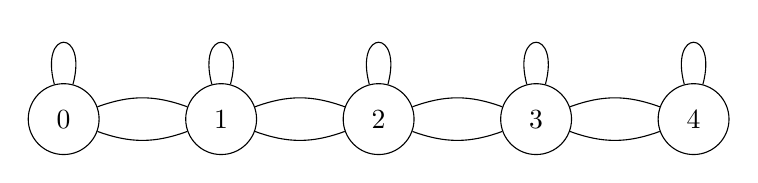
\begin{tikzpicture}[scale=1, every node/.style={circle, draw, minimum size=9mm}]
                    % Nodes
                    \node (n0) at (0,0) {0};
                    \node (n1) at (2,0) {1};
                    \node (n2) at (4,0) {2};
                    \node (n3) at (6,0) {3};
                    \node (n4) at (8,0) {4};

                    % Self-loops (simple arcs above each node)
                    \draw (n0) to[loop above] (n0);
                    \draw (n1) to[loop above] (n1);
                    \draw (n2) to[loop above] (n2);
                    \draw (n3) to[loop above] (n3);
                    \draw (n4) to[loop above] (n4);

                    % Bilateral edges between neighbors (two simple lines: one up, one down)
                    % 0 <-> 1
                    \draw (n0) to[bend left=20] (n1);
                    \draw (n1) to[bend left=20] (n0);
                    % 1 <-> 2
                    \draw (n1) to[bend left=20] (n2);
                    \draw (n2) to[bend left=20] (n1);
                    % 2 <-> 3
                    \draw (n2) to[bend left=20] (n3);
                    \draw (n3) to[bend left=20] (n2);
                    % 3 <-> 4
                    \draw (n3) to[bend left=20] (n4);
                    \draw (n4) to[bend left=20] (n3);
                \end{tikzpicture}
            \end{center}
            We never see a drawing, but \code{dsp} stores exactly this connectivity. Then:
            \begin{itemize}
                \item \code{sparisty\_pattern.copy\_from(dsp)} freezes it in a compressed format;
                \item And \code{system\_matrix.reinit(sparisty\_pattern)} allocates numeric storage \emph{only} for those $(i, j)$.
            \end{itemize}
        \end{examplebox}
        \newpage
        \item \textbf{Freeze the graph into a compressed pattern (CSR-like)}:
        \begin{lstlisting}[language=C++]
sparsity_pattern.copy_from(dsp);\end{lstlisting}
        Converts that flexible graph into a compact, cache-friendly layout (row-compressed). This step is all about \textbf{memory efficiency and fast access} downstream.

        \item \textbf{Create global Stiffness Matrix $A$}:
        \begin{lstlisting}[language=C++]
system_matrix.reinit(sparsity_pattern);\end{lstlisting}
        Where \code{sparsity\_pattern} tells which entries $(i,j)$ are allowed to exist. After this, the matrix has the right shape and memory allocated, but its entries are all zero.
        
        \item \textbf{Right-hand side}:
        \begin{lstlisting}[language=C++]
system_rhs.reinit(dof_handler.n_dofs());\end{lstlisting}
        Initializes the \textbf{right-hand side vector} $f$. Its size equals the number of global unknowns (DoFs). This vector will later be filled with the load term integrals $\displaystyle\int f \varphi_{i}$. In other words, it is the input forcing vector for the linear system.

        \item \textbf{Create Solution vector}:
        \begin{lstlisting}[language=C++]
solution.reinit(dof_handler.n_dofs());\end{lstlisting}
        Initializes the \textbf{solution vector} $u$. Same size as \code{system\_rhs}. At the beginning, it is just a vector of zeros. After solving, it will contain the approximate solution at each DoF. In other words, it is the unknown vector that will store the result after the solver runs.
    \end{itemize}
\end{enumerate}
After setup, we are ready to assemble the system: $Au = f$.
\begin{itemize}
    \item \code{system\_matrix}: $A$
    \item \code{solution}: $u$
    \item \code{system\_rhs}: $f$
\end{itemize}

\begin{center}
    \href{https://gist.github.com/AndreVale69/f04f312da68d16c253f46493ae7eaf24#file-poisson1d-cpp}{\faIcon{download} Source}
    \hspace{1em}
    \qrcode{https://gist.github.com/AndreVale69/f04f312da68d16c253f46493ae7eaf24#file-poisson1d-cpp}
\end{center}

\noindent
Output:
\begin{lstlisting}
===============================================
Setup started
Initializing the mesh
  Number of elements = 40
  Mesh saved to mesh-40.vtk
-----------------------------------------------
Initializing the finite element space
  Degree                     = 1
  DoFs per cell              = 2
  Quadrature points per cell = 2
-----------------------------------------------
Initializing the DoF handler
  Number of DoFs = 41
-----------------------------------------------
Initializing the linear system
  Initializing the sparsity pattern
  Initializing the system matrix
  Initializing the system right-hand side
  Initializing the solution vector\end{lstlisting}